\chapter{Results \& Discussion}\label{chap:results}

In this chapter, the results of the experiments are presented and discussed. The experiments were conducted to evaluate the generalization performance of four GNN architectures on 49 graph classification datasets. The four neural network architectures described in Chapter \ref{chap:experiments}. The datasets using for training and testing are described in Section \ref{sec:datasets}. The experiments were conducted using the training and testing procedures described in Section \ref{sec:Experimental procedures}.

The following sections present the results of the experiments. First, the graph parameters calculated for the datasets are shown in~\ref{sec:result_graph_parameters}. Then, the generalization error of the four GNN architectures is presented individually in~\ref{sec:result_gcn},~\ref{sec:result_sgc},~\ref{sec:result_gatv2}, and~\ref{sec:result_mpnn}. Finally, the correlation analysis between the generalization error and the graph parameters is discussed in each section.

Note that, the correlation analysis for each architecture is presented with two scatter plots. One contains all datasets, and the other contains only datasets with more than 1000 graphs. The reason for this separation is that the datasets with fewer graphs tend to have higher variability in generalization error, which can lead to misleading correlations.

\section{Graph parameters}~\label{sec:result_graph_parameters}

The graph parameters calculated in the experiments are shown in Table \ref{tab:gp1}~\ref{tab:gp2}. 

TODO: some datasets have 0 as the result, need to mention that

\section{Graph Convolutional Networks}~\label{sec:result_gcn}
The calculated generalization error of the experiments using Graph Convolutional Networks are shown in Table~\ref{tab:ge_gcn}.


\begin{table}[!ht]
    \centering
    \footnotesize
    \begin{tabular}{p{3.5cm}|p{5cm}p{5cm}}
    \hline
    \toprule
        Name & Ave. generalization error & Standard deviation \\ 
    \midrule
        AIDS & 0.0081874905154109 & 0.0117165874689817 \\ 
        BZR & 0.0708846226334571 & 0.0609733723104 \\ 
        BZR\_MD & 0.0961788743734359 & 0.1091229766607284 \\ 
        COLORS-3 & 0.06828124076128 & 0.0298492461442947 \\ 
        COX2 & 0.0840000063180923 & 0.1163316890597343 \\ 
        COX2\_MD & 0.0750205665826797 & 0.1105385944247245 \\ 
        DD & 0.0138164404779672 & 0.0569455623626709 \\ 
        DHFR & 0.1413267403841018 & 0.0572429783642292 \\ 
        DHFR\_MD & 0.0547252781689167 & 0.1071747243404388 \\ 
        ENZYMES & 0.1968750059604644 & 0.1035036742687225 \\ 
        ER\_MD & 0.0477907545864582 & 0.0669434815645217 \\ 
        FRANKENSTEIN & 0.0549374930560588 & 0.0326129123568534 \\ 
        KKI & 0.1822761297225952 & 0.3100946843624115 \\ 
        MCF-7 & 0.0019999979995191 & 0.0135001158341765 \\ 
        MCF-7H & 0.003406238509342 & 0.0127300517633557 \\ 
        MOLT-4 & 0.0015624940861016 & 0.0123682264238595 \\ 
        MOLT-4H & 0.0034062266349792 & 0.0167727246880531 \\ 
        MUTAG & 0.1002193242311477 & 0.0946124866604805 \\ 
        Mutagenicity & 0.040156252682209 & 0.0229900479316711 \\ 
        NCI-H23 & 0.0028750181663781 & 0.0120867453515529 \\ 
        NCI-H23H & 0.0005312621360644 & 0.0108473878353834 \\ 
        NCI1 & 0.0832187384366989 & 0.0319501645863056 \\ 
        NCI109 & 0.0711562559008598 & 0.0383276790380477 \\ 
        OHSU & 0.3857143521308899 & 0.2356772273778915 \\ 
        OVCAR-8 & 0.0038125098217278 & 0.0155245345085859 \\ 
        OVCAR-8H & 0.0028437494765967 & 0.0162141937762498 \\ 
        P388 & 0.0043125031515955 & 0.013600654900074 \\ 
        P388H & 0.0070000053383409 & 0.0142645183950662 \\ 
        PC-3 & 0.0024375021457672 & 0.0098565947264432 \\ 
        PC-3H & 0.0060312449932098 & 0.0117860734462738 \\ 
        PROTEINS\_full & 0.0026662945747375 & 0.0525967963039875 \\ 
        PTC\_FM & 0.0923068895936012 & 0.1087017878890037 \\ 
        PTC\_FR & 0.1018810272216796 & 0.1225867569446563 \\ 
        PTC\_MM & 0.088215485215187 & 0.0875236690044403 \\ 
        PTC\_MR & 0.0782608613371849 & 0.0882423818111419 \\ 
        Peking\_1 & 0.2760869860649109 & 0.2045421004295349 \\ 
        SF-295 & 0.0032500028610229 & 0.0157351642847061 \\ 
        SF-295H & 0.0017812550067901 & 0.0091287596151232 \\ 
        SN12C & 0.0003750085888896 & 0.0128499586135149 \\ 
        SN12CH & 0.0031250000465661 & 0.0179813411086797 \\ 
        SW-620 & 0.0014062583213672 & 0.0130064394325017 \\ 
        SW-620H & 0.0014687419170513 & 0.0133227882906794 \\ 
        SYNTHETIC & 0.0120833460241556 & 0.0160114392638206 \\ 
        SYNTHETICnew & 0.1366666555404663 & 0.1849549412727356 \\ 
        Synthie & 0.1234375014901161 & 0.0413857623934745 \\ 
        UACC257 & 0.0011249959934502 & 0.0108615579083561 \\ 
        UACC257H & 0.000843757414259 & 0.0126192783936858 \\ 
        Yeast & 0.0053749978542327 & 0.027795847505331 \\ 
        YeastH & 0.0001875102461781 & 0.0135009009391069 \\ 
    \end{tabular}
    \caption{Generalization error of the GCN model on 49 datasets}
    \label{tab:ge_gcn} % ge -> generalization error
\end{table}

The correlation between the generalization error and the graph parameters are shown in Figure~\ref{fig:correlation_GCN} and Figure~\ref{fig:correlation_ignore_less_than_1000_GCN}.

\begin{figure}[H]
    \centering
    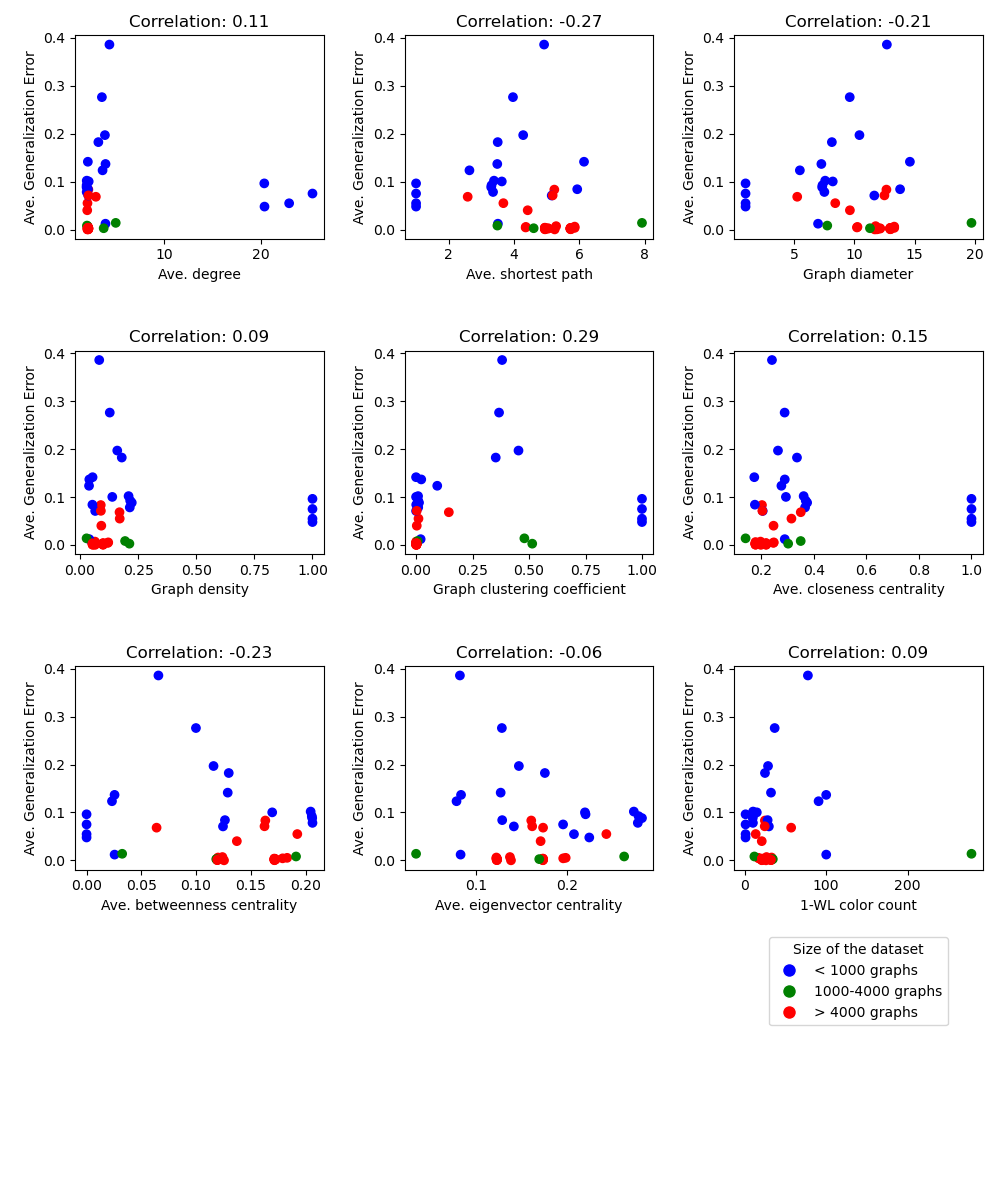
\includegraphics[width=\textwidth]{images/correlation_GCN.png}
    \caption{Scatter plots showing the relationship between various graph parameters and the average generalization error of Graph Convolutional Networks (GCNs). Each subplot presents the correlation coefficient between a specific graph parameter and the generalization error. Colors indicate dataset sizes: blue (<1000 graphs), red (1000-4000 graphs), and green (>4000 graphs).}
    \label{fig:correlation_GCN}
\end{figure}

\begin{figure}[H]
    \centering
    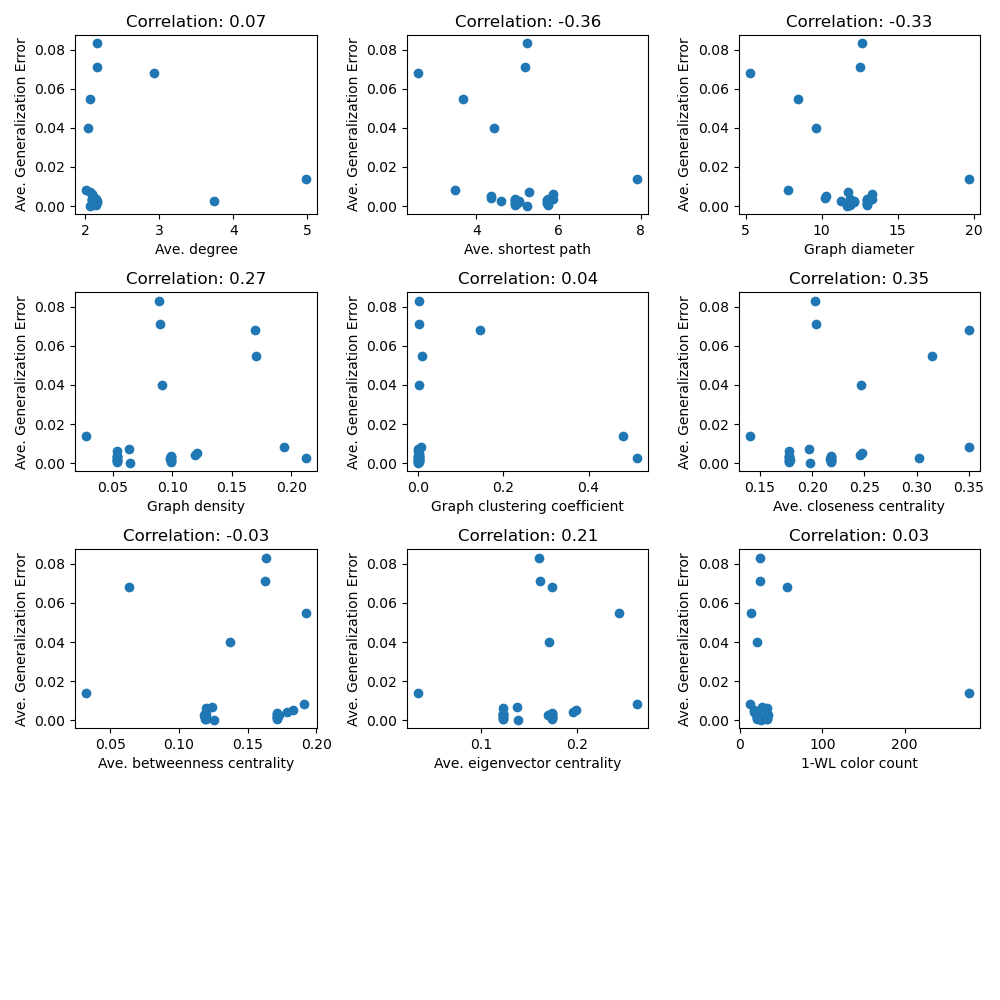
\includegraphics[width=\textwidth]{images/correlation_ignore_less_than_1000_GCN.png}
    \caption{Scatter plots showing the relationship between various graph parameters and the average generalization error of Graph Convolutional Networks (GCNs). Each subplot presents the correlation coefficient between a specific graph parameter and the generalization error. Only datasets with more than 1000 graphs are considered. There are 40 datasets in this plot and another 19 datasets are not included.}
    \label{fig:correlation_ignore_less_than_1000_GCN}
\end{figure}


% -------------------------------------------------------------------------------------------------

\subsection{Discussion}

The experimental results presented with \ref{fig:correlation_GCN} and \ref{fig:correlation_ignore_less_than_1000_GCN}  above demonstrate the relationships between graph parameters and the average generalization error across datasets of varying sizes. It gives insights into how different graph parameters influence the generalization performance of Graph Convolutional Networks (GCNs) in graph classification tasks. The following observations are noted from the results:

\subsubsection{Correlation Analysis}

\paragraph{Negative Correlations with Graph Diameter and Shortest Path}
The results indicate a moderate negative correlation between generalization error and both graph diameter (-0.21) and average shortest path (-0.27) in the full dataset analysis~\ref{fig:correlation_GCN}. When considering only larger datasets~\ref{fig:correlation_ignore_less_than_1000_GCN}, these correlations become stronger (-0.33 and -0.36, respectively), suggesting that GNNs generalize better on graphs with shorter path lengths and smaller diameters. 

\paragraph{Influence of Graph Density and Clustering Coefficient}
The correlation with graph density is relatively weak (0.09 in the full dataset~\ref{fig:correlation_GCN}, 0.27 in the filtered dataset~\ref{fig:correlation_ignore_less_than_1000_GCN}), but the clustering coefficient shows a higher correlation of 0.29 in the full dataset, which drops to 0.04 in the filtered dataset. This suggests that clustering coefficient may influence generalization, but likely due to the higher noise levels in smaller samples, the effect diminishes when excluding small datasets. On the contrary, the graph density indicate a moderate positive correlation in the filtered dataset, which is not observed in the full dataset.


\paragraph{Centrality Measures}
Closeness centrality shows a consistent positive correlation with generalization error (0.15 in the full dataset, 0.35 in the filtered dataset). On the other hand, betweenness centrality has a moderate negative correlation (-0.23 in the full dataset, -0.03 in the filtered dataset). Eigenvector Centrality shows weak correlations in both cases (-0.06 and 0.21). Overall, if the dataset size is considered, closeness centrality and eigenvector centrality appear to have a moderate positive influence on generalization error, while betweenness centrality has a negative effect.

\paragraph{1-WL Color Count}
The correlation with 1-WL color count is relatively weak (0.09 and 0.03 in full and filtered datasets, respectively). This finding is interesting, as it indicates that while the Weisfeiler-Lehman test is commonly used as a measure of GNN expressiveness, it does not necessarily dictate generalization behavior, for the GCN model at least.

\subsubsection{Summary}
Overall, structural features like average shortest path, graph diameter, and  centrality measure have stronger relationships with generalization error compared to measures like 1-WL color count and potentially clustering coefficient. Nonetheless, none of the parameters shows a highly significant correlation.
% -------------------------------------------------------------------------------------------------

\section{Simplified Graph Convolution}~\label{sec:result_sgc}
The calculated generalization error of the experiments using Simplified Graph Convolution are shown in Table~\ref{tab:ge_sgc}.


\begin{table}[!ht]
    \centering
    \footnotesize
    \begin{tabular}{p{3.5cm}|p{5cm}p{5cm}}
    \hline
    \toprule
        Name & Ave. generalization error & Standard deviation \\ 
    \midrule
        AIDS & 0.0094999792054295 & 0.0067623262293636 \\
        BZR & 0.0398076958954334 & 0.0535244457423687 \\
        BZR\_MD & 0.1050406470894813 & 0.095137633383274 \\
        COLORS-3 & 0.0739687532186508 & 0.0297187566757202 \\
        COX2 & 0.0861333459615707 & 0.0670665428042411 \\
        COX2\_MD & 0.0440740659832954 & 0.1867186874151229 \\
        DD & 0.1082454919815063 & 0.0635362416505813 \\
        DHFR & 0.1035643592476844 & 0.0682980865240097 \\
        DHFR\_MD & 0.0555799715220928 & 0.1178753077983856 \\
        ENZYMES & 0.1837499886751175 & 0.0857001841068267 \\
        ER\_MD & 0.0475622005760669 & 0.0829107165336608 \\
        FRANKENSTEIN & 0.061875008046627 & 0.0329361073672771 \\
        KKI & 0.0291044823825359 & 0.2818436622619629 \\
        MCF-7 & 0.000656247138977 & 0.0137401102110743 \\
        MCF-7H & 0.001156234764494 & 0.0151891019195318 \\
        MOLT-4 & 0.0018124937778338 & 0.0116189513355493 \\
        MOLT-4H & 0.0018437386024743 & 0.0139454510062932 \\
        MUTAG & 0.1163011640310287 & 0.0678915232419967 \\
        Mutagenicity & 0.0481875017285347 & 0.0258940625935792 \\
        NCI-H23 & 0.0031250119209289 & 0.0100476266816258 \\
        NCI-H23H & 5.9604645663569045e-09 & 0.0108693270012736 \\
        NCI1 & 0.0839374884963035 & 0.0166628845036029 \\
        NCI109 & 0.0677187517285347 & 0.0309047140181064 \\
        OHSU & 0.0270329676568508 & 0.2689114809036255 \\
        OVCAR-8 & 0.0021875083912163 & 0.0154096204787492 \\
        OVCAR-8H & 0.0021250010468065 & 0.0172242671251297 \\
        P388 & 0.0042812586762011 & 0.0127577884122729 \\
        P388H & 0.0118749979883432 & 0.0183747168630361 \\
        PC-3 & -0.0001562476099934 & 0.0097229816019535 \\
        PC-3H & 0.000968748354353 & 0.0120369335636496 \\
        PROTEINS\_full & 0.0114296078681945 & 0.0617067217826843 \\
        PTC\_FM & 0.101800300180912 & 0.1584279388189315 \\
        PTC\_FR & 0.102684274315834 & 0.0604767650365829 \\
        PTC\_MM & 0.1027272716164588 & 0.1311521083116531 \\
        PTC\_MR & 0.1173060312867164 & 0.1128198280930519 \\
        Peking\_1 & 0.232065200805664 & 0.290688544511795 \\
        SF-295 & 0.0006874978425912 & 0.0154270688071846 \\
        SF-295H & 0.0021562576293945 & 0.0088528767228126 \\
        SN12C & 0.001562523888424 & 0.0126561466604471 \\
        SN12CH & -6.249547004699707e-05 & 0.0126207722350955 \\
        SW-620 & 0.0008437514188699 & 0.0120212435722351 \\
        SW-620H & 0.0024687468539923 & 0.0140694072470068 \\
        SYNTHETIC & 0.0154166761785745 & 0.0234100967645645 \\
        SYNTHETICnew & 0.1204166635870933 & 0.0984339192509651 \\
        Synthie & 0.1784375011920929 & 0.0635749474167823 \\
        UACC257 & 3.124475551885553e-05 & 0.0105321435257792 \\
        UACC257H & 5.9604645663569045e-09 & 0.0123304584994912 \\
        Yeast & 0.0027187527157366 & 0.0283915027976036 \\
        YeastH & 0.0021875023376196 & 0.0149637833237648 \\
    \end{tabular}
    \caption{Generalization error of the SGC model on 49 datasets}
    \label{tab:ge_sgc} % ge -> generalization error
\end{table}

The correlation between the generalization error and the graph parameters are shown in Figure~\ref{fig:correlation_SGC} and Figure~\ref{fig:correlation_ignore_less_than_1000_SGC}.

\begin{figure}[H]
    \centering
    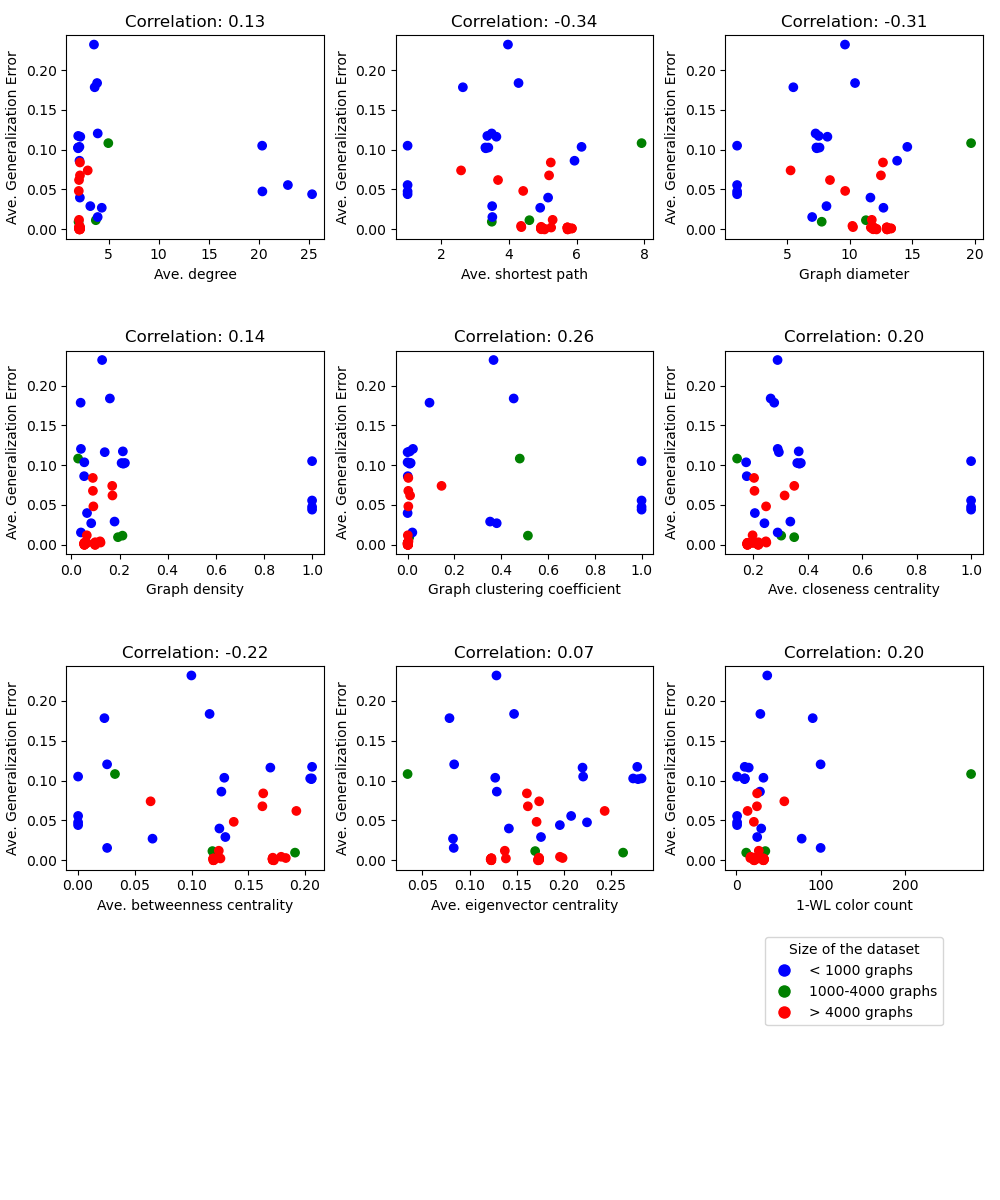
\includegraphics[width=\textwidth]{images/correlation_SGC.png}
    \caption{Scatter plots showing the relationship between various graph parameters and the average generalization error of a Simplified Graph Convolution (SGC) model. Each subplot presents the correlation coefficient between a specific graph parameter and the generalization error. Colors indicate dataset sizes: blue (<1000 graphs), red (1000-4000 graphs), and green (>4000 graphs).}
    \label{fig:correlation_SGC}
\end{figure}

\begin{figure}[H]
    \centering
    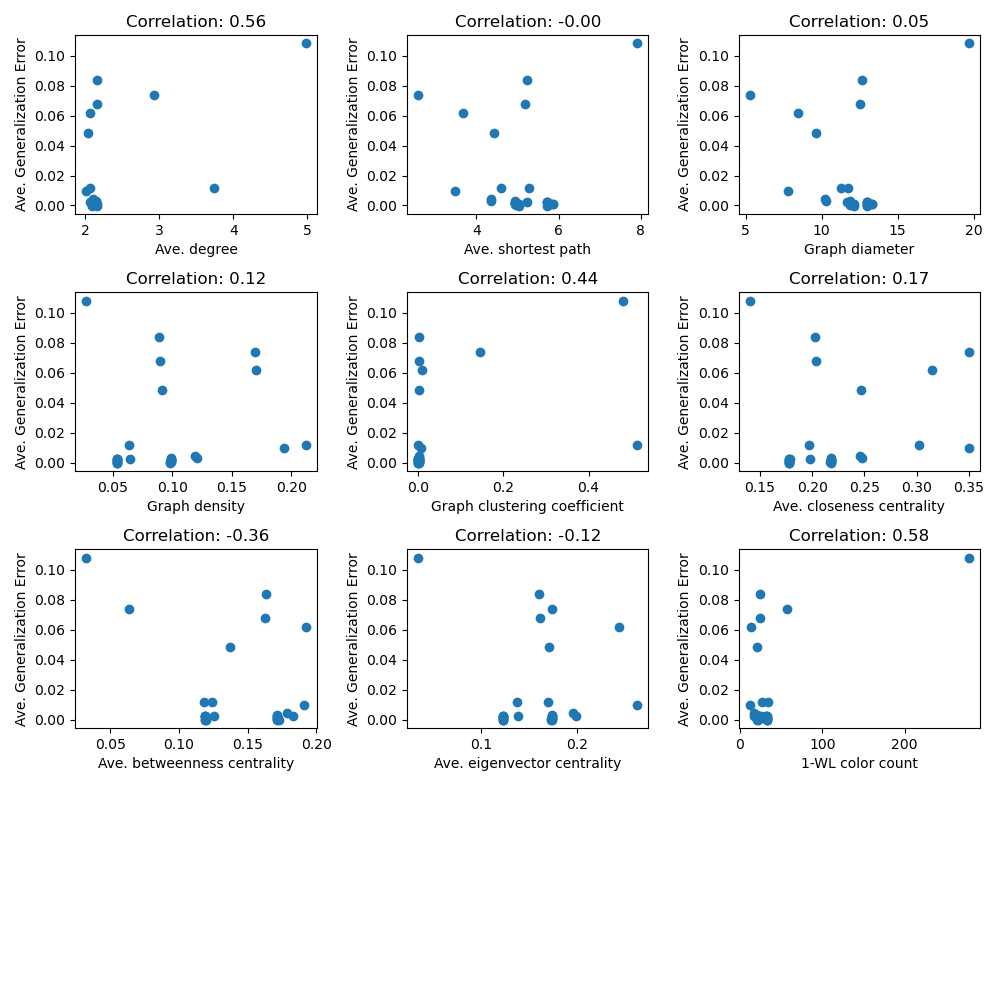
\includegraphics[width=\textwidth]{images/correlation_ignore_less_than_1000_SGC.png}
    \caption{Scatter plots showing the relationship between various graph parameters and the average generalization error of a Simplified Graph Convolution (SGC) model. Each subplot presents the correlation coefficient between a specific graph parameter and the generalization error. Only datasets with more than 1000 graphs are considered. There are 40 datasets in this plot and another 19 datasets are not included.}
    \label{fig:correlation_ignore_less_than_1000_SGC}
\end{figure}

\subsection{Discussion}

The experimental results presented with \ref{fig:correlation_SGC} and \ref{fig:correlation_ignore_less_than_1000_SGC}  above demonstrate the relationships between graph parameters and the average generalization error across datasets of varying sizes. It gives insights into how different graph parameters influence the generalization performance of Simplified Graph Convolution (SGC) in graph classification tasks. The following observations are noted from the results:

\subsubsection{Correlation Analysis}

\paragraph{Graph Average Degree}
The average degree shows a weak positive correlation with generalization error in the full dataset (0.13), which increases substantially to a strong correlation (0.56) when only datasets with more than 1000 graphs are considered. This implies that generalization error is more sensitive to average degree in larger graph datasets. The weak correlation in the full dataset may be due to noise introduced by smaller datasets.

\paragraph{Graph Diameter and Shortest Path}
Both graph diameter (-0.31) and average shortest path (-0.34) exhibit moderate negative correlations with generalization error in the full dataset, indicating that datasets with more compact graph structures (smaller diameters and shorter path lengths) tend to generalize better. Interestingly, these correlations diminish in the filtered dataset to 0.05 and -0.00, respectively. It suggests that the significance of these measures decreases due to larger size of datasets. 

\paragraph{Graph Density and Clustering Coefficient}
The clustering coefficient shows a moderate positive correlation with generalization error in both datasets (0.26 in the full dataset and 0.44 in the filtered dataset). This indicates that generalization error increases in denser neighborhoods, particularly in larger datasets. Graph density, on the other hand, shows weak correlations in both cases (0.14 in the full dataset and 0.12 in the filtered dataset). It suggests a weaker effect on generalization behavior compared to clustering coefficient.

\paragraph{Centrality Measures}
Among the centrality measures, betweenness centrality exhibits negative correlations with generalization error (-0.22 in the full dataset and -0.36 in the filtered dataset). This indicates that higher betweenness centrality leads to lower generalization error, particularly in larger datasets. Closeness centrality and eigenvector centrality exhibit weak to moderate correlations (0.20 and 0.07 in the full dataset; 0.17 and -0.12 in the filtered dataset), comparing to the betweenness centrality. Overall, centrality measures have a weak to moderate influence on generalization error, with betweenness centrality showing the most significant effect.

\paragraph{1-WL Color Count}
The 1-WL color count demonstrates a weak positive correlation with generalization error in the full dataset (0.20), which becomes substantially stronger in the filtered dataset (0.58). It suggests that the expressiveness of the graph structure, as measured by 1-WL color count, plays a more significant role in generalization behavior in larger datasets.

\subsubsection{Summary}
The results indicate that structural features like average degree and clustering coefficient are more predictive of generalization behavior in larger datasets, as reflected by their stronger correlations in the filtered dataset. In contrast, graph parameters like average graph diameter and shortest path, which show moderate correlations in the full dataset, diminish as the dataset size increases. Centrality measures, particularly betweenness centrality, exhibit a more consistent relationship with generalization error, with stronger correlations in the filtered dataset. Lastly, 1-WL coloring number shows the most significant correlation with generalization error, indicating that the expressiveness of the graph structure plays an important role in generalization ability.

\section{Graph Attention Networks v2}~\label{sec:result_gatv2}
The calculated generalization error of the experiments using Graph Convolutional Networks are shown in Table~\ref{tab:ge_gatv2}.

\begin{table}[!ht]
    \centering
    \footnotesize
    \begin{tabular}{p{3.5cm}|p{5cm}p{5cm}}
    \hline
    \toprule
        Name & Ave. generalization error & Standard deviation \\ 
    \midrule
    AIDS & 0.0043124915100634 & 0.0093050524592399 \\ 
    BZR & 0.0609999969601631 & 0.0820248797535896 \\ 
    BZR\_MD & 0.0472357682883739 & 0.1092826277017593 \\ 
    COLORS-3 & 0.043281253427267 & 0.0240429937839508 \\ 
    COX2 & 0.0630377084016799 & 0.0825407281517982 \\ 
    COX2\_MD & 0.085967056453228 & 0.0940771996974945 \\ 
    DD & 0.1108267903327941 & 0.0513695515692234 \\ 
    DHFR & 0.1174587234854698 & 0.0517340935766696 \\ 
    DHFR\_MD & 0.0339438319206237 & 0.1088754534721374 \\ 
    ENZYMES & 0.2141666859388351 & 0.0753771364688873 \\ 
    ER\_MD & 0.0706957802176475 & 0.0536176972091198 \\ 
    FRANKENSTEIN & 0.0540624968707561 & 0.0219314694404602 \\ 
    KKI & 0.2389925420284271 & 0.3365208804607391 \\ 
    MCF-7H & 0.0001249790220754 & 0.0124741122126579 \\ 
    MCF-7 & 0.0007500052452087 & 0.0141399931162595 \\ 
    MOLT-4H & 0.0006562412017956 & 0.0142586100846529 \\ 
    MOLT-4 & 0.0004374861600808 & 0.0111289750784635 \\ 
    MUTAG & 0.0780701860785484 & 0.0887901559472084 \\ 
    Mutagenicity & 0.0441875047981739 & 0.0323983952403068 \\ 
    NCI-H23H & 5.9604645663569045e-09 & 0.0108693270012736 \\ 
    NCI-H23 & 9.377002425026149e-05 & 0.0100130606442689 \\ 
    NCI109 & 0.087562508881092 & 0.0293439049273729 \\ 
    NCI1 & 0.079031229019165 & 0.0203865990042686 \\ 
    OHSU & 0.2868131995201111 & 0.3649870157241821 \\ 
    OVCAR-8H & 6.25073880655691e-05 & 0.0174949076026678 \\ 
    OVCAR-8 & 0.0003125071525573 & 0.0130370762199163 \\ 
    P388H & 0.0005312621360644 & 0.0131217204034328 \\ 
    P388 & 0.0042187571525573 & 0.0145163964480161 \\ 
    PC-3H & -5.9604645663569045e-09 & 0.0116321872919797 \\ 
    PC-3 & 0.0003437519189901 & 0.0097120413556694 \\ 
    PROTEINS\_full & 0.0294719096273183 & 0.0491058491170406 \\ 
    PTC\_FM & 0.0593364052474498 & 0.0939571186900138 \\ 
    PTC\_FR & 0.0619827024638652 & 0.0776680409908294 \\ 
    PTC\_MM & 0.0872390493750572 & 0.1021735519170761 \\ 
    PTC\_MR & 0.0601662322878837 & 0.0595390647649765 \\ 
    Peking\_1 & 0.250543475151062 & 0.2304597347974777 \\ 
    SF-295H & 5.9604645663569045e-09 & 0.0102338008582592 \\ 
    SF-295 & 0.0002187669306294 & 0.0146516626700758 \\ 
    SN12CH & 0.0 & 0.0145929940044879 \\ 
    SN12C & 0.0006562650087289 & 0.0130099598318338 \\ 
    SW-620H & 0.0002187490463256 & 0.0138334389775991 \\ 
    SW-620 & 0.0002812623861245 & 0.0136981671676039 \\ 
    SYNTHETIC & 0.0212500095367431 & 0.0290307682007551 \\ 
    SYNTHETICnew & 0.1174999922513961 & 0.0795870795845985 \\ 
    Synthie & 0.1574999988079071 & 0.1155846491456031 \\ 
    UACC257H & 5.9604645663569045e-09 & 0.0123304584994912 \\ 
    UACC257 & 0.0005000054952688 & 0.0106954481452703 \\ 
    YeastH & 0.0011562525760382 & 0.0136780375614762 \\ 
    Yeast & 0.0016562461387366 & 0.0281631872057914 \\ 
    \end{tabular}
    \caption{Generalization error of the GATv2 model on 49 datasets}
    \label{tab:ge_gatv2} % ge -> generalization error
\end{table}


The correlation between the generalization error and the graph parameters are shown in Figure~\ref{fig:correlation_GATv2} and Figure~\ref{fig:correlation_ignore_less_than_1000_GATv2}.

\begin{figure}[H]
    \centering
    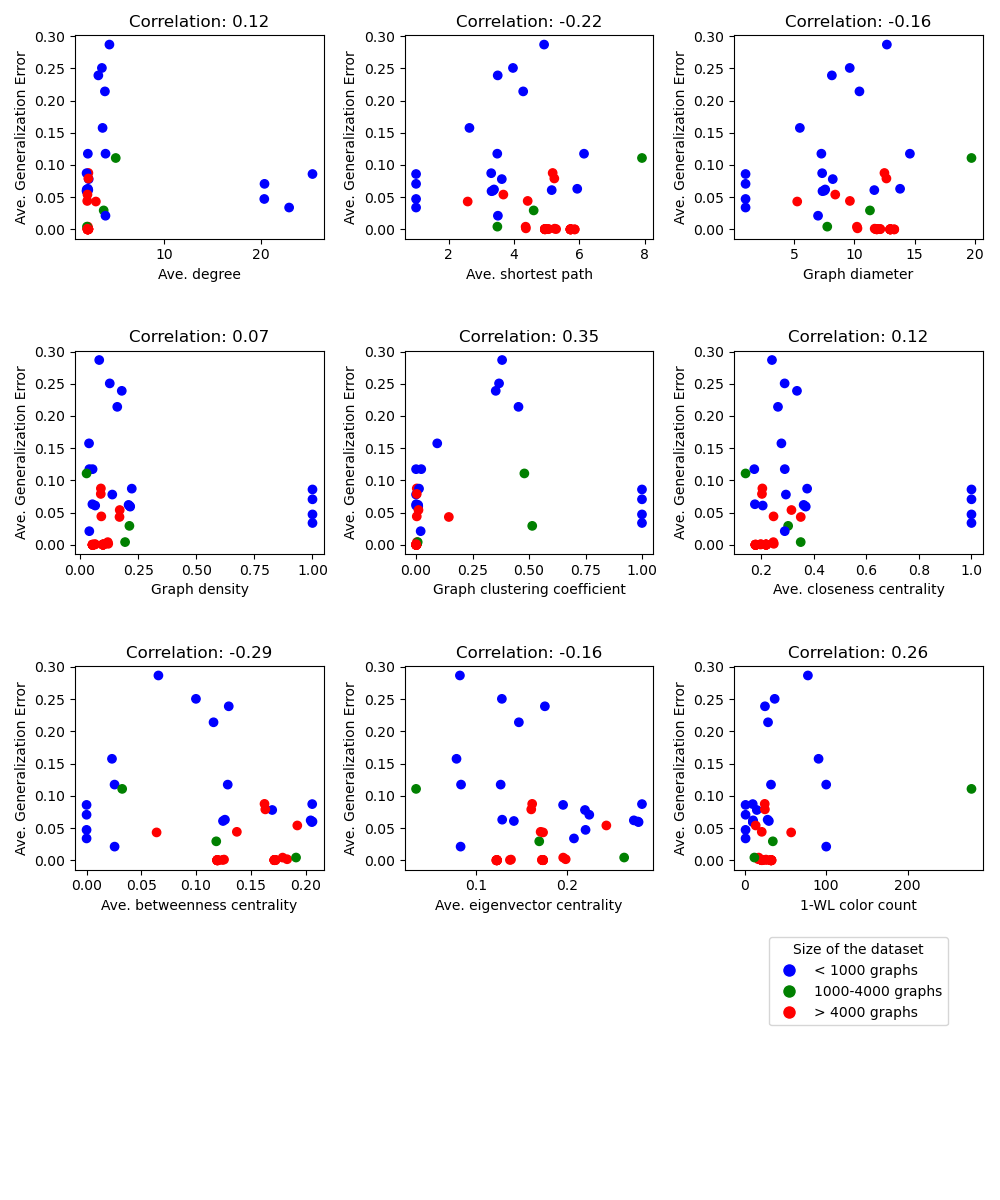
\includegraphics[width=\textwidth]{images/correlation_GATv2.png}
    \caption{Scatter plots showing the relationship between various graph parameters and the average generalization error of Graph Attention Networks v2 (GATv2). Each subplot presents the correlation coefficient between a specific graph parameter and the generalization error. Colors indicate dataset sizes: blue (<1000 graphs), red (1000-4000 graphs), and green (>4000 graphs).}
    \label{fig:correlation_GATv2}
\end{figure}

\begin{figure}[H]
    \centering
    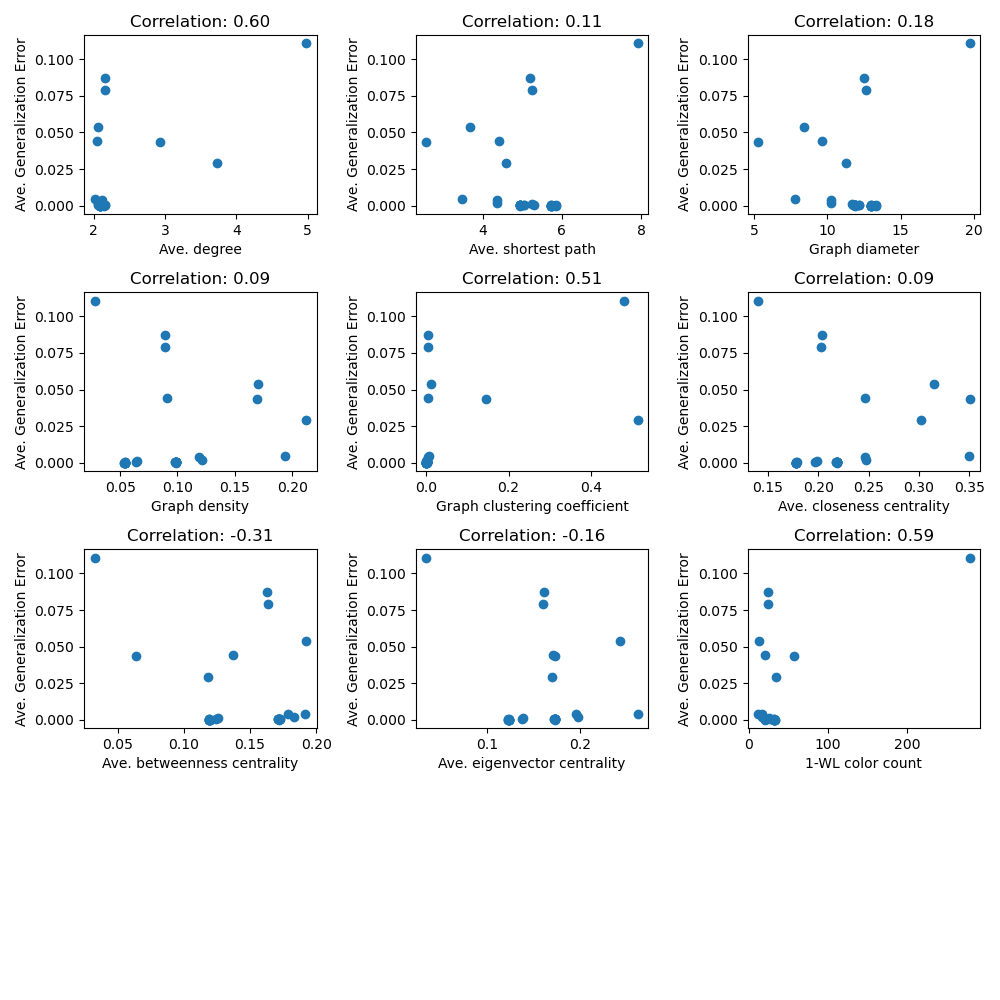
\includegraphics[width=\textwidth]{images/correlation_ignore_less_than_1000_GATv2.png}
    \caption{Scatter plots showing the relationship between various graph parameters and the average generalization error of Graph Attention Networks v2 (GATv2). Each subplot presents the correlation coefficient between a specific graph parameter and the generalization error. Only datasets with more than 1000 graphs are considered. There are 40 datasets in this plot and another 19 datasets are not included.}
    \label{fig:correlation_ignore_less_than_1000_GATv2}
\end{figure}

\subsection{Discussion}

The experimental results presented with \ref{fig:correlation_GATv2} and \ref{fig:correlation_ignore_less_than_1000_GATv2} above demonstrate the relationships between graph parameters and the average generalization error across datasets of varying sizes. It gives insights into how different graph parameters influence the generalization performance of Graph Attention Networks v2 (GATv2) in graph classification tasks. The following observations are noted from the results:

\subsubsection{Correlation Analysis}

\paragraph{Average Degree}
A weak positive correlation of 0.12 between average degree and generalization error is observed in the full dataset analysis (\ref{fig:correlation_GATv2}). This correlation becomes significantly stronger (0.60) in the larger datasets (\ref{fig:correlation_ignore_less_than_1000_GATv2}), indicating that higher average degree may negatively impact generalization. This trend suggests that increased connectivity might lead to reduce the model's ability to effectively generalize to unseen data.

\paragraph{Shortest Path and Graph Diameter}
In the full dataset, a negative correlation is noted between generalization error and both shortest path (-0.22) and graph diameter (-0.16), indicating that smaller and more compact graphs are associated with better generalization. However, in larger datasets, the negative correlation with the shortest path diminishes (0.11), while graph diameter shows a weak positive correlation (0.18). My interpretation is that the noise in smaller datasets may have influenced the initial negative correlations.

\paragraph{Graph Density and Clustering Coefficient}
Graph density shows a very weak correlation in the full dataset (0.07) and remains weak in larger datasets (0.09). On the other hand, the clustering coefficient demonstrates considerable variability, with a strong positive correlation of 0.35 in the full dataset, which increases further (0.51) in the filtered dataset. This suggests the clustering coefficient has more impact on generalization than graph density, particularly in larger datasets.

\paragraph{Centrality Measures}
Betweenness centrality exhibits a moderate negative correlation (-0.29) in the full dataset and has similar correlation in the filtered dataset (-0.31). The average eigenvector centrality has also a negative correlation (-0.16 both in the full dataset and the filtered dataset), but relatively weaker than betweenness centrality. Closeness centrality, however, has a weak positive correlation (0.12 in the full dataset, 0.09 in the filtered dataset), indicating little impact on generalization error. It is the weakest among the centrality measures. 

\paragraph{1-WL Color Count}
The 1-WL color count demonstrates moderate positive correlation in the full dataset (0.26), but this correlation increases significantly in larger datasets (0.59). It is similar to the results observed in the SGC model, suggesting that the expressiveness of the graph structure plays a more significant role in generalization behavior in larger datasets.

\subsubsection{Summary}
The results indicate that structural features like average degree and clustering coefficient are more predictive of generalization behavior in larger datasets, as reflected by their stronger correlations in the filtered dataset. In contrast, graph parameters like average graph diameter and shortest path, which show moderate negative correlations in the full dataset, but it becomes weak positive correlations in the filtered dataset. One possible explanation is that the noise in smaller datasets may have influenced the initial negative correlations. Centrality measures, particularly betweenness centrality, exhibit a more consistent relationship with generalization error, with stronger correlations in the filtered dataset. Lastly, 1-WL coloring number shows the most significant correlation with generalization error, indicating that the expressiveness of the graph structure plays an important role in generalization ability.

\section{Message Passing Neural Networks}~\label{sec:result_mpnn}